\documentclass[12pt]{article}
\usepackage{geometry}
\usepackage{amsmath}
\usepackage{amssymb}
\usepackage{enumitem}
\usepackage{fancyhdr}
\usepackage{tikz}
\usepackage{color}
\usepackage{xspace}
\usepackage{thumbpdf}
\usepackage{listings}
\usepackage{verbatim}
\usepackage{hyperref}
\usepackage{booktabs}
\usepackage{colortbl}
\usetikzlibrary{trees}
\pagestyle{fancy}

\newcommand{\xref}[1]{\S\ref{#1}}
\definecolor{darkred}{rgb}{0.7,0,0}
\definecolor{darkgreen}{rgb}{0,0.5,0}
\hypersetup{colorlinks=true,
	linkcolor=darkred,
	citecolor=darkgreen}

\lstset{
	basicstyle=\ttfamily,
	mathescape
}

\lstdefinestyle{customc}{
	belowcaptionskip=1\baselineskip,
	breaklines=true,
	% xleftmargin=20pt,
	language=matlab,
	% frame=L,
	escapeinside={@}{@},
	showstringspaces=false,
	basicstyle=\small\ttfamily,
	keywordstyle=\bfseries\color{green!40!black},
	commentstyle=\itshape\color{purple!40!black},
	%identifierstyle=\color{blue},
	stringstyle=\color{orange},
	% directivestyle=\color{brown},
	%numbers=left,
	%numberstyle=\tiny\color{gray}
}

\lstdefinestyle{customctable}{
	aboveskip=-\medskipamount,
	belowskip=-\medskipamount,
	language=C,
	escapeinside={@}{@},
	showstringspaces=false,
	basicstyle=\scriptsize\ttfamily,
	keywordstyle=\bfseries\color{green!40!black},
	commentstyle=\itshape\color{purple!40!black},
	%identifierstyle=\color{blue},
	stringstyle=\color{orange},
	directivestyle=\color{brown},
}

\textheight=8.5in

\newcommand{\hongzi}[1]{{{\color{red}(HM: #1)}}}

\lhead{6.854 Pset 3}
\chead{Hongzi Mao  \: \footnotesize{collaborators:} Calvin Lee, Linus Hamilton}
\rhead{Spet 28, 2016}

\begin{document}
	
\section*{Problem 1}

Modify \textsc{Count-Min} by setting parameter $\epsilon=1/k$, $b = \frac{3}{\epsilon} = \frac{3}{1/k} = 3k$ and $l = O(log\: m)$. Then probability of failure using Union Bound is $1/3$, and the space required is $O(k\:log(m)\:log(n))$. Detailed analysis as follows.

Recall in \textsc{Count-Min}, in a \emph{single} vector, by setting size $b = 3/\epsilon$ and $\epsilon = 1/k$, the probability for the (one-way only) error term to exceed $\epsilon n = n/k$ is 
\begin{equation*}
Pr[Y_x > \epsilon n] \leq \frac{E[Y_x]}{\epsilon n} \leq \frac{n/b}{\epsilon n} = \frac{1}{3}.
\end{equation*}

Augmenting $l = O(log\:\frac{m}{1/3}) = O(log\:m)$ of such vectors, we reduce such probability to $1/3^l$. Then by union bounding over $m$ different items, we have for probability at lest $1-1/3=2/3$, that the estimated frequency $\hat{f_x}$ of item $x$ yields
\begin{equation*}
\hat{f_x} \approx f_x \pm \frac{n}{k},
\end{equation*}
w.r.t. true frequency $f_x$, for \emph{all} elements $x$ in the universe of size $m$.

Thus, with probability $2/3$, the error of estimated frequency of all items are bounded by $\frac{n}{k}$, which results in a correct set of overstocked items. Notice in \textsc{CMS} vector, each entry requires $O(log\:n)$ bits to represent the number of items currently stored. Therefore, the total space required in terms of bits is $O(b\:l\:log(n)) = O(3k\:log(\frac{m}{1/3})\:log(n)) = O(k\:log(m)\:log(n))$.

\pagebreak

\section*{Problem 2}
\paragraph{(a)}
Argue this via contradiction. Suppose after seen half of the stream, we are \emph{unable} to determine the set of distinct elements it has seen so far, by looking into the internal state of the algorithm. Then in the second half of the stream, the algorithm would have no way to tell if an element appears is outside the distinct set or not. This way, an adversary can always design a pattern of elements that fail the algorithm. In the second half of the algorithm, even if it perfectly tracks the distinct set of the element (there could be mistakes because it lost track of the first half), it lost the distinct elements that only appears in the first half. 

Therefore, in order to deterministically count the exact number of distinct items, the first half of the algorithm must be able to output the set of distinct element seen so far. Because the items come in the first half can be \emph{all} distinct, the logarithm must be able to remember all the elements in the first half. Now without loss of generality, the first `half' may just be the entire stream, therefore the algorithm has to remember all the elements it has seen. 

\paragraph{(b)} The algorithm must have at least $N$ internal states to deterministically solve the exact distinct elements problem. This is because in the worst case, the element in the stream can be all distinct and by part (a) we know we have to remember all of them. Therefore the algorithm needs $N$ internal states in order to do so. 

\paragraph{(c)} Each internal state costs at least $O(log(m))$ bits of the space because we don't know in a priori which element from the universe $m$ will show up but we need to store them distinctly. Also, from part (a) and part (b), we then need $\Omega(N \cdot log(m))$ bits of space.

\pagebreak

\section*{Problem 3} 
\paragraph{(a)} We derive the space upper bound by providing an algorithm that solves the problem with upper bound $O(|V|log|V|)$ bit of space.

\subparagraph{Algorithm} We associate a group and and opposite group for each vertex $v$. Every time a new edge $E$ connecting vertex $v_1$ and $v_2$ is seen from the array, we check if $v_1$ $v_2$ belong to the same group, which breaks the rule of bipartite graph. Upon seeing new edge, the opposite group of $v_1$ will be set as the group of $v_2$ and vice versa. In such process, new group may be recorded, or existing groups may be merged. Specifically, the following pseudocode shows the steps of checking, 

\begin{lstlisting}[style=customc]
  for $E(v_1, v_2)$ in edge_stream:  % streaming
    if $v_1$.group exists:
      
      if $v_2$.group exists:
        if $v_1$.group == $v_2$.group:
          return non-bipartite
        else  % merge
          for $v$ in $v_2$.opposite_group:
            $v$.group := $v_1$.group
            $v$.opposite_group := $v_1$.opposite_group
          end for
          for $v$ in $v_2$.group:  % need cache to prevent overwrite
            $v$.group := $v_1$.opposite_group
            $v$.opposite_group := $v_1$.group
          end for
        end if
      
      else:  % $v_2$ is new, add it to group
        $v_2$.group := $v_1$.opposite_group
        $v_2$.opposite_group := $v_1$.group
      
      end if 
    
    else:  % $v_1$ is new
      if $v_2$.group exists:
        $v_1$.group := $v_2$.opposite_group 
        $v_1$.opposite_group := $v_2$.group
        
      else:  % $v_1$ and $v_2$ are both new
        $v_1$.group := new_group_1
        $v_2$.group := new_group_2
        $v_1$.opposite_group := $v_2$.group
        $v_2$.opposite_group := $v_1$.group
      end if
    end if
  end for
  
  return bipartite
\end{lstlisting}

\subparagraph{Analysis} The streaming algorithm makes sure that there is no edge connection between nodes in the same group, which returns \emph{non-bipartite} in the first clause. If this is not violated, it means edges are only across groups, we can output two merged groups by putting each two sub-groups on the two sides, which results in \emph{bipartite}. In the \emph{merge} step, we make sure the opposite group of all nodes in a group are the same, and going the opposite group, all the nodes have their opposite groups pointing back. This ensures a \emph{single} checking of no edges in the same group is sufficient when seeing a new edge. 

Notice that there can be at most as many groups as the number of vertices, therefore the space complexity is bounded by $O(|V|log|V|)$ bit of space\footnote{However this algorithm does not necessarily give a good upper bound regarding the time complexity}. 

\paragraph{(b)} In order to determine whether a streaming edge set constructs a bipartite under adversarial order, the algorithm has to remember all the vertices  it has seen. Otherwise, the adversary can give the algorithm the vertex that it misses (also the edges connecting it, as we lost \emph{all} information of such vertex) in any of the group, which results in bipartite or non-bipartite graph. But the algorithm cannot determine between the two cases because it does not store the information of that adversary vertex. 

As there are $|V|$ vertices, storing any one of them requires $O(log|V|)$ bits of space. Therefore, storing all vertices requires $\Omega(|V|log|V|)$ bits of space in total.

\pagebreak

\section*{Problem 4}
\paragraph{(a)} False. In Figure \ref{fig:4}(a), all edges have distinct capacity. The bottleneck link is right before sink node $t$, making the max flow $1$. However, the flow can go through both upper or lower part of the graph with value $1$.
\paragraph{(b)} False. In Figure \ref{fig:4}(b), the original graph has max-flow value 2. However, adding the opposite link will make the max-flow value 11.
\paragraph{(c)} False. In Figure \ref{fig:4}(c), the min cut was originally on two links with capacity $1$, which makes the max-flow value $2$. However, when adding $\lambda=2$ capacity on all links, the min-cut becomes the link with new capacity $5$.
\paragraph{(d)} False. In Figure \ref{fig:4}(d), if $s$ is the source, $t$ is the sink, then the flow value is $1$. If $t$ is the source, $u$ is the sink, then the flow value is also $1$. However, if $s$ is the source, $u$ is the sink, the flow value can become $2$.
\begin{figure}
	\centering
	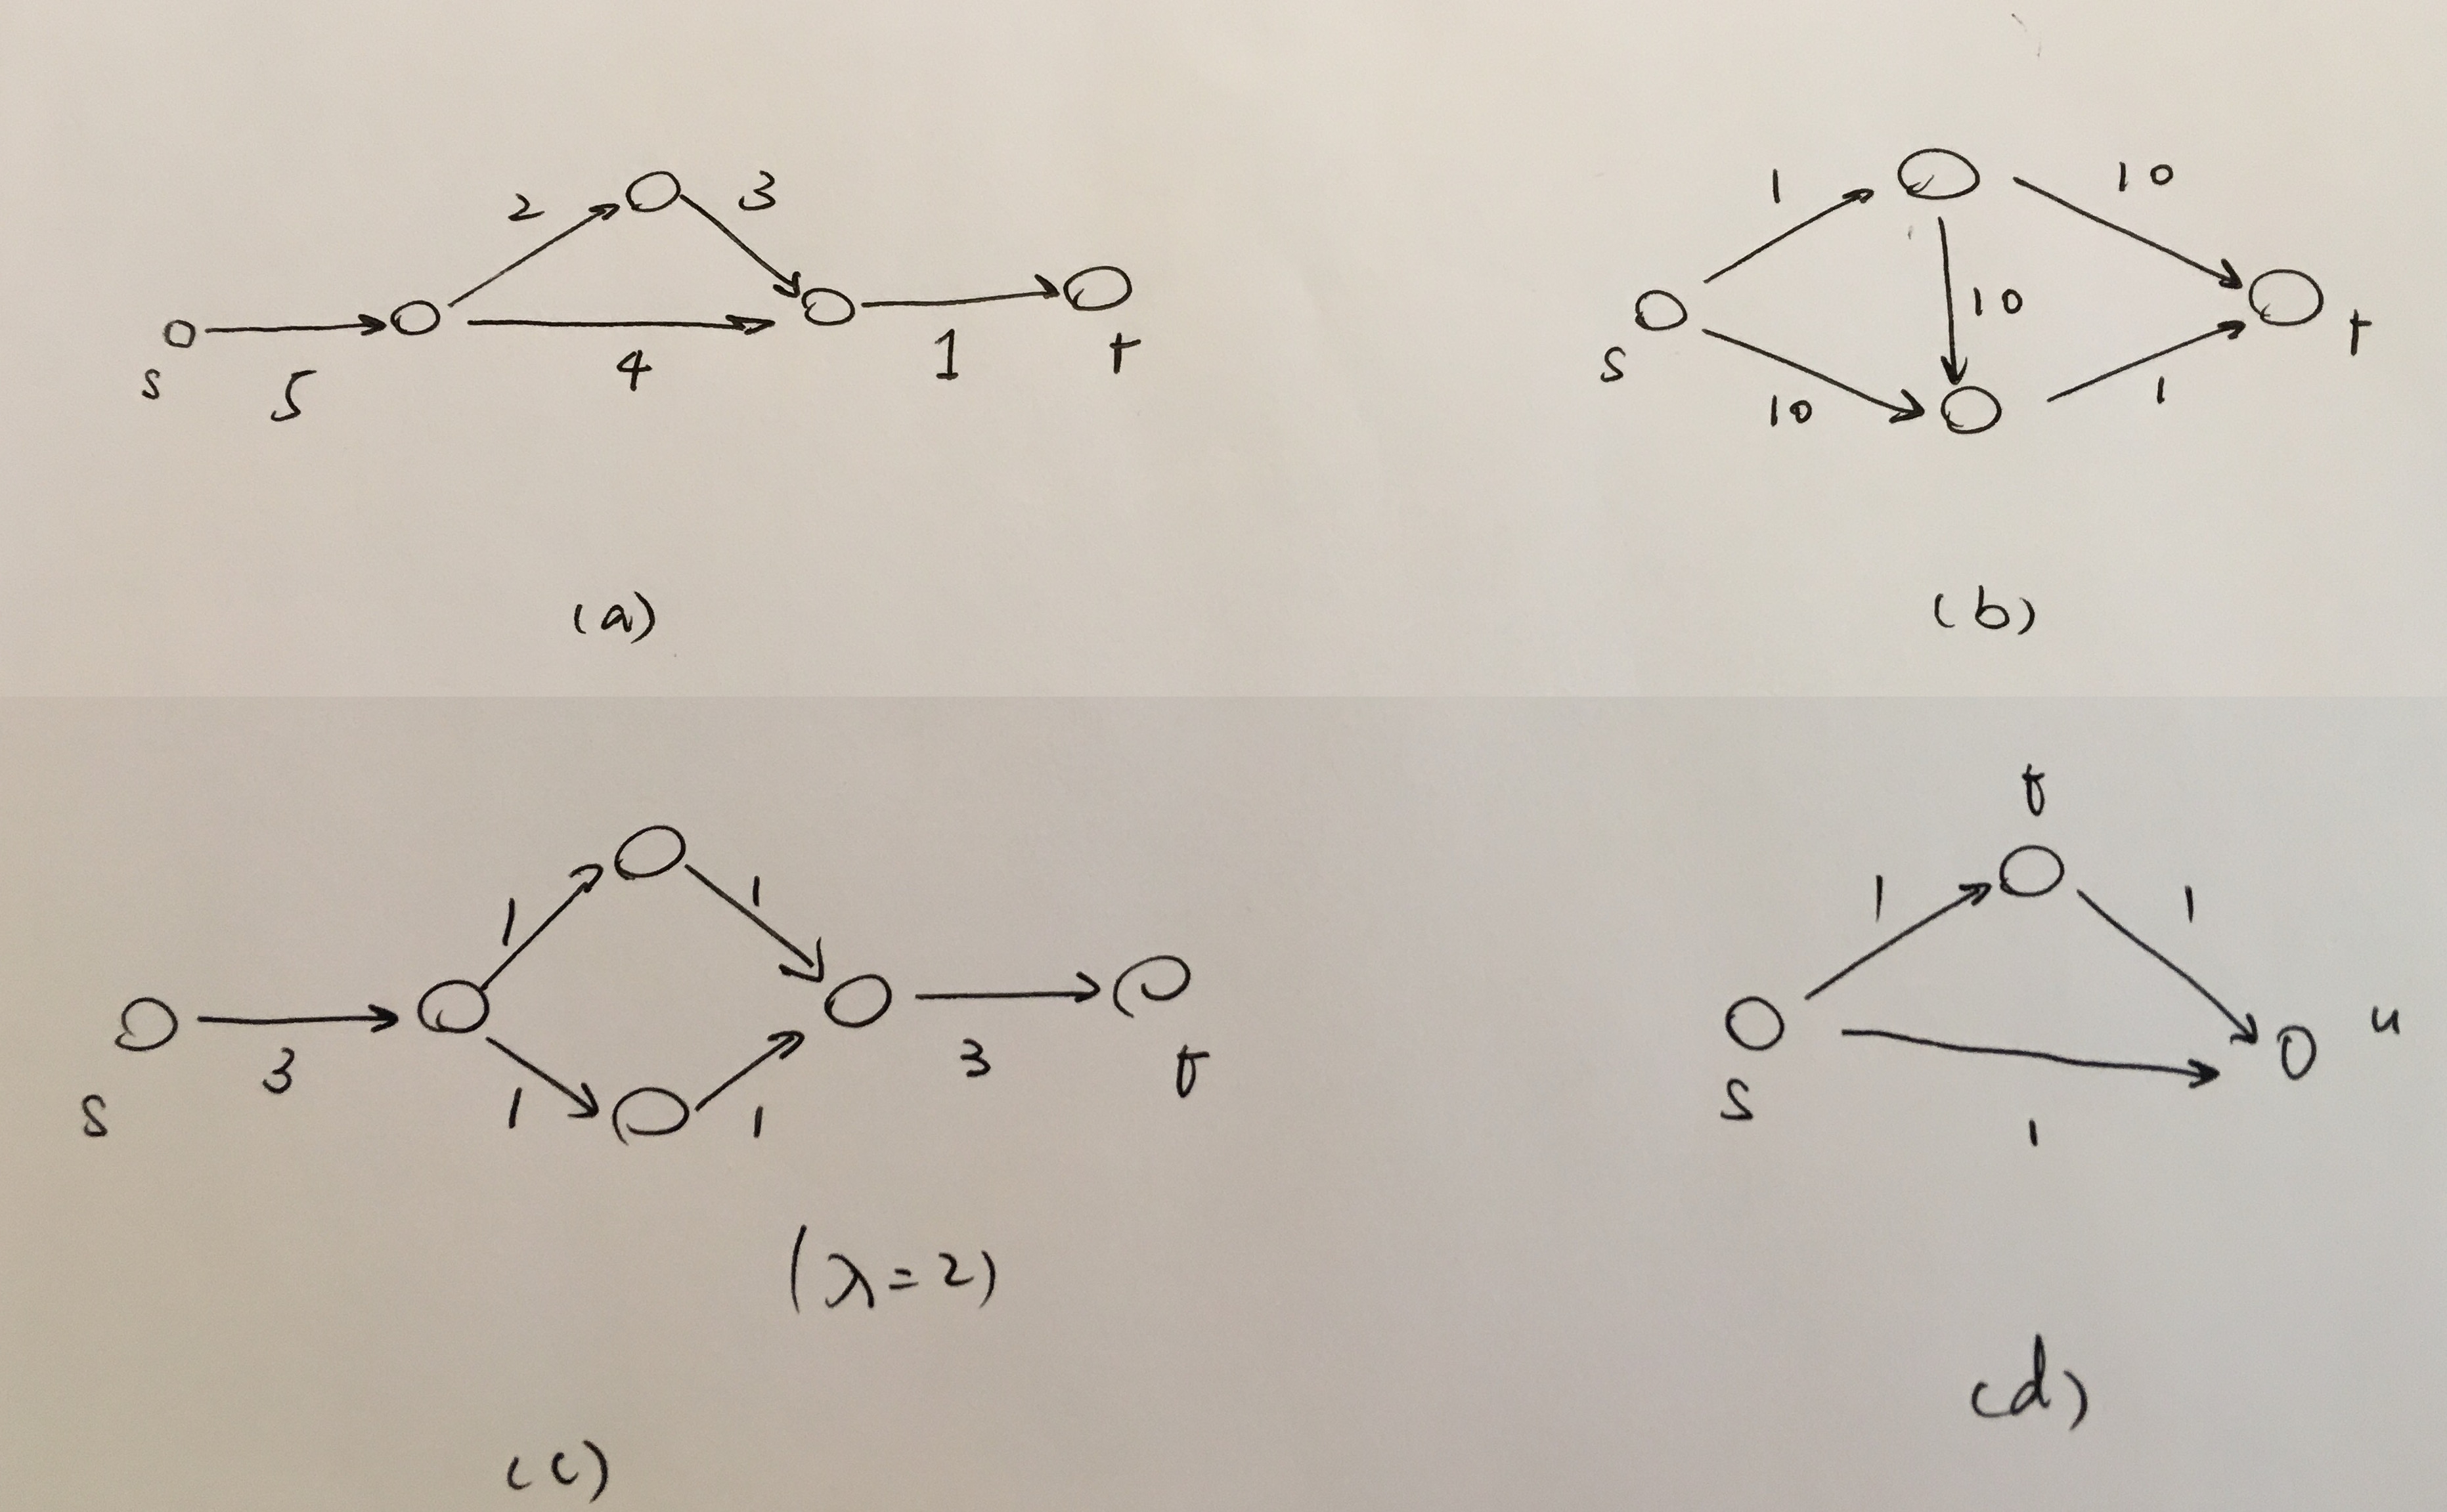
\includegraphics[width=1\textwidth]{4.jpg}
	\caption{Illustration of the graphs.} \label{fig:4}
\end{figure}
\section*{Problem 5}
\subparagraph{Algorithm}
Illustrated in Figure \ref{fig:5}, we represent the problem as a max-flow problem. We create two layers in between the artificial source and sink. The first layer is consist of nodes of $q_{i,j}$, where $i<j$ and RedSox is removed from $i$ and $j$. The edge connecting $s$ and each $q_{i,j}$ node has capacity $q_{i,j}$. Then, the second layer is made up from all teams except RedSox. Next, connect an edge between node $q_{i,j}$ and team $i$, as well as an edge between node $q_{i,j}$ and team $j$, both with capacity $q_{i,j}$. Finally, connecting all team nodes to the sink node. For each team $i$, the capacity of the edge to the sink is $w[\text{RedSox}] + \sum_j g_{\text{RedSox}, j} - w[i]$ \footnote{If the winning team needs \emph{strictly} more winning games, we need this capacity to be $w[\text{RedSox}] + \sum_j g_{\text{RedSox}, j} - w[i] - 1$}, denoting how many games at most it can win, such that RedSox still wins more games than it. 

During the construction of the graph, if any of the edge from the second layer to the sink is negative, we then immediately terminate the program with conclusion that RedSox can not win the pennant. After the graph is constructed, we run the max-flow algorithm. If the max-flow result equals to $\sum_{i<j, i, j \neq \text{RedSox}} q_{i,j}$, we conclude that RedSox is possible to win the pennant. If not, then RedSox is bumped up.

\subparagraph{Analysis} The graph is constructed in this way such that each unit of flow through a node in the last layer can be viewed as this team node wins a game. Different layers in the flow graph put different constraints of the problem. (1) The connection between the last layer and the sink confines the maximum number of games this team can win, given that the total number of winning games is less than RedSox, assuming RedSox wins all remaining games. If an edge value is negative during construction, it means this team already wins more games than RedSox even if RedSox wins all remaining games, which thus means RedSox is impossible to win. (2) The connection from sink to the second layer confines the total number of remaining games a team can win (the sum of winning game of $i$ and $j$ is confined to be $q_{i,j}$). Under (1) and (2), if the maximum flow is $\sum_{i<j, i, j \neq \text{RedSox}} q_{i,j}$, it means all constraints are satisfied (not exceeding the capacity) and all remaining games are played. This means RedSox is possible to have more winning games than others in some configuration, if it wins all its remaining games. Otherwise, even if RedSox wins all remaining games, some other team still has more winning games than it.

Given an efficient max-flow algorithm, this adaptation can solve this problem efficiently in the sense that the complexity is in the scale of total $q_{ij}$ for all $i$ and $j$, namely the extra construction in the graph does not exceed the scale of total $q_ij$ (which connects all team nodes, therefore not exceeding the scale of total number of teams).

\begin{figure}
	\centering
	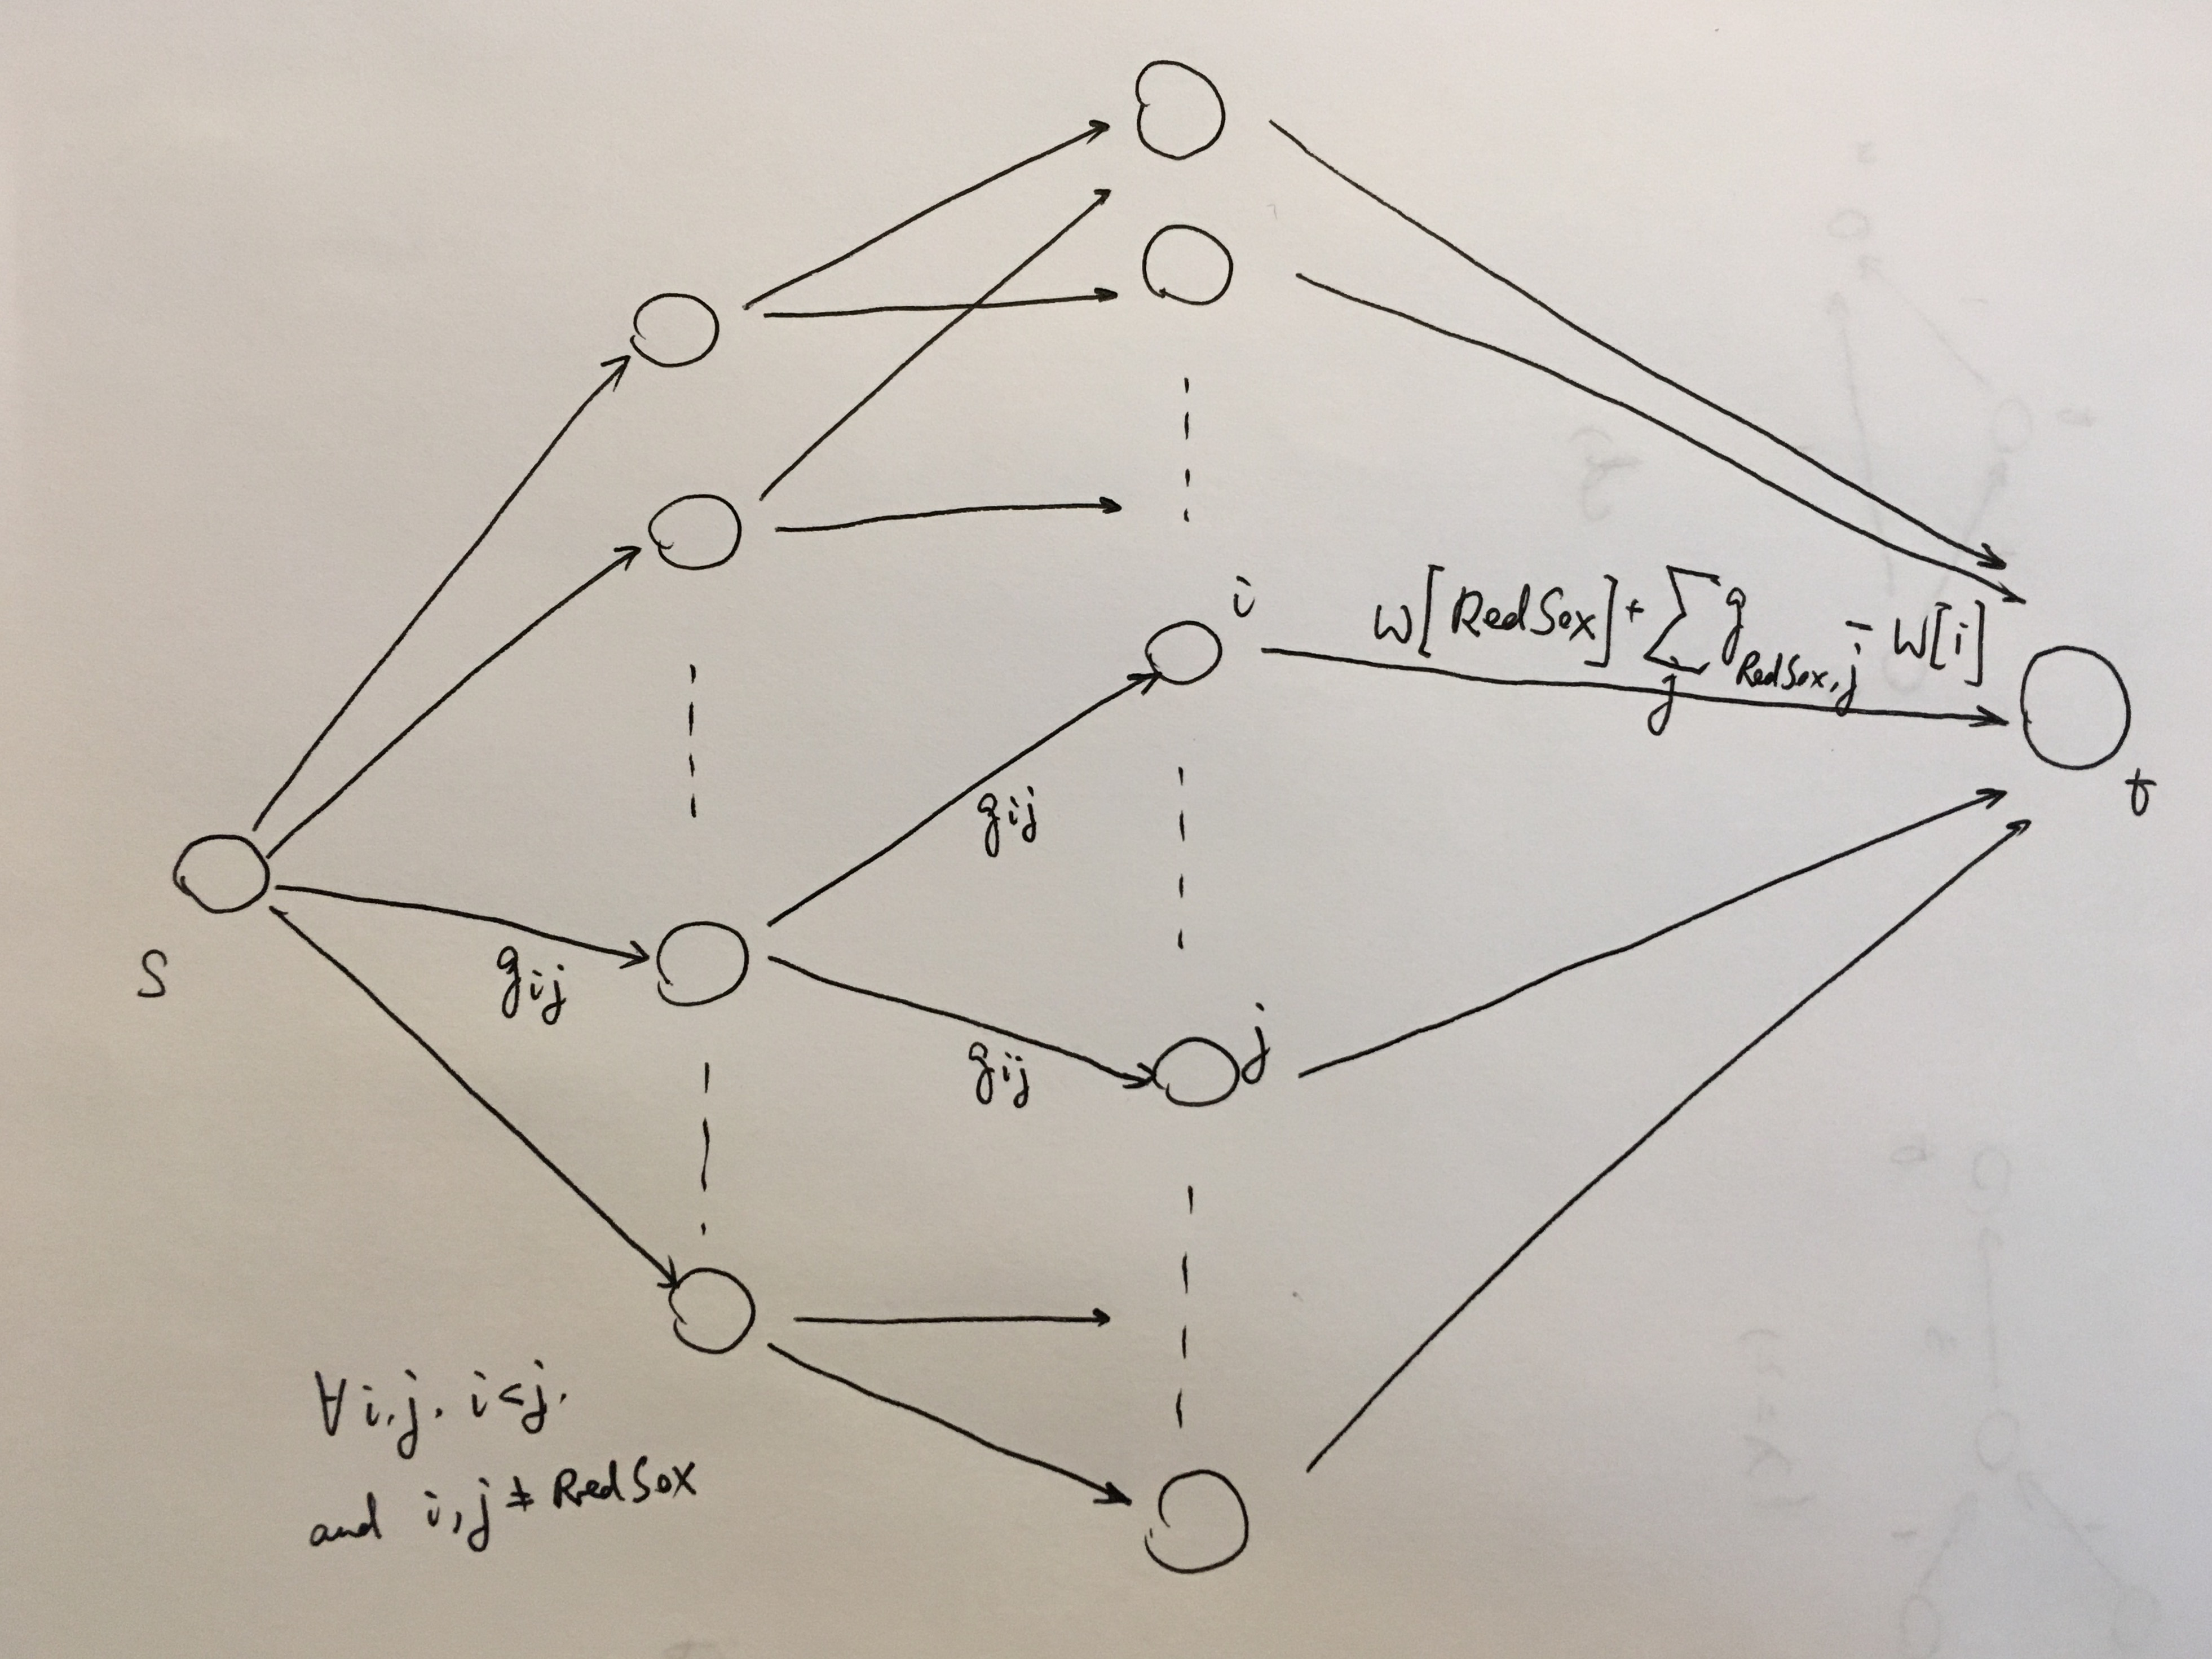
\includegraphics[width=0.85\textwidth]{5.jpg}
	\caption{Flow-based algorithm for the American League.} \label{fig:5}
\end{figure}

\pagebreak
.
\pagebreak

\section*{Problem 6}
\paragraph{(a)}
Recall that \emph{Johnson-Lindenstrauss Lemma} states, for any set of $m$ $n$-dimensional vectors $x^1, ..., x^m \in \mathbb{R}^n$, and any $1/2 \geq \epsilon >0$, there exists an $k$-by-$n$ matrix $D$, with $k = O(\epsilon^{-2}\:log\:n)$, such that 
\begin{equation*}
(1-\epsilon) ||x^i - x^j||^2_2 \leq ||D x^i - D x^j||^2_2 \leq (1+\epsilon) ||x^i - x^j||^2_2,
\end{equation*}
for any $i$ and $j$.

Similar to $\ell_2$ norm dimension reduction above, for vectors $x^1, ..., x^m \in \mathbb{R}^n$, we can find a matrix $C$, with dimension $k$-by-$n$, such that $||x||_{B^TC^TCB}$ approximately preserves A-norm\footnote{Note that $A$ is square shaped and has dimension $n$-by-$n$.} of $||x||_A$, where $A=B^TB$, 
\begin{equation*}
(1-\epsilon) ||x^i - x^j||^2_A \leq ||x^i - x^j||^2_{B^TC^TCB} \leq (1+\epsilon) ||x^i - x^j||^2_A.
\end{equation*}

Also similar to the construction of matrix $D$ in the class, we argue that if we make each entry in matrix $C$ follow the distribution $\mathcal{N}(0, \frac{1}{k})$, and it suffices to show
\begin{equation*}
Pr\left[(1-\epsilon) ||x||^2_A \leq ||x||^2_{B^TC^TCB} \leq (1+\epsilon) ||x||^2_A\right] \geq 1 - \frac{1}{n^3}.
\end{equation*}

\subparagraph{Proof}
Let
\begin{equation*}
Y_i := \left(C(Bx)\right)_i = \sum_{j=1}^n C_{ij} (Bx)_j. 
\end{equation*}

The distribution of $Y_i$ thus yields,
\begin{equation*}
Y_i \sim \sum_{j=1}^n \mathcal{N}(0, \frac{1}{k}) (Bx)_j = \mathcal{N}(0, \frac{||Bx||_2}{k}). 
\end{equation*}

Then we have
\begin{align*}
Pr\left[\left|||x||^2_{B^TC^TCB} - ||x||^2_A\right| > \epsilon ||x||^2_A\right] &= Pr\left[\left|||Bx||^2_{C^TC} - ||Bx||^2_2\right| > \epsilon ||Bx||^2_2\right] \\
&= Pr\left[\left|\sum_i^k Y_i^2 - ||Bx||_2^2\right| > \epsilon ||Bx||^2_2\right] \\
&= Pr\left[\left|\sum_i^k \left(\frac{\sqrt{k}}{||Bx||_2}Y_i\right)^2 - k\right| > \epsilon k\right]\\
&\left(\text{Notice that} \frac{\sqrt{k}}{||Bx||_2}Y_i \sim \mathcal{N}(0,1)\right)\\
&\underset{{\text{Chernoff}}}{\leq} 2\:\text{exp}\left(-\frac{k\epsilon^2}{8}\right) \\
&\underset{{k = O(\epsilon^{-2}\:log\:n)}}{\leq} \frac{1}{n^3}.
\end{align*}

Therefore the norm preservation property similarly holds for $A$-norm. $\square$
\paragraph{(b)} We will show below that the norm preservation compression for $\ell_\infty$ norm yields $k \geq n$, which breaks the Lemma's bound\footnote{One can break the bound by viewing $\epsilon$ as fixed and then group $n$ arbitrarily.} of $k = O(\epsilon^{-2}log\:n)$. We show this via a set of vectors as a counter-example. The idea is sketched in Figure \ref{fig:6-2}.

Construct $n$ vectors: $(1, 0, 0, ..., 0), \: \: (0, 1, 0, ..., 0), \: \: (0, 0, 1, ..., 0), \: \: ..., \: \: (0, 0, 0, ..., 1)$. Compressing these vector down to vectors in $\mathbb{R}^k$, while preserving the $\ell_\infty$ norm (which takes max of all the entries), requires the resulting vectors to have at least one entry $1 \pm \epsilon$. 

Assuming $k < n$, by Pigeon-Hole principle, we can find two entries from the set of $n$ vectors, such that their compressed vectors have the same entry with $1 \pm \epsilon$ colliding. Now because the transformation is assumed to be linear, we can add the original two vector up, which results in a $\ell_\infty$ norm equals to 1 still, but adding the compressed vectors up results in $\ell_\infty$ norm equals to $2 \pm 2\epsilon$. This breaks the norm preservation under linear transformation, therefore we conclude that we need $k \geq n$.

\begin{figure}
	\centering
	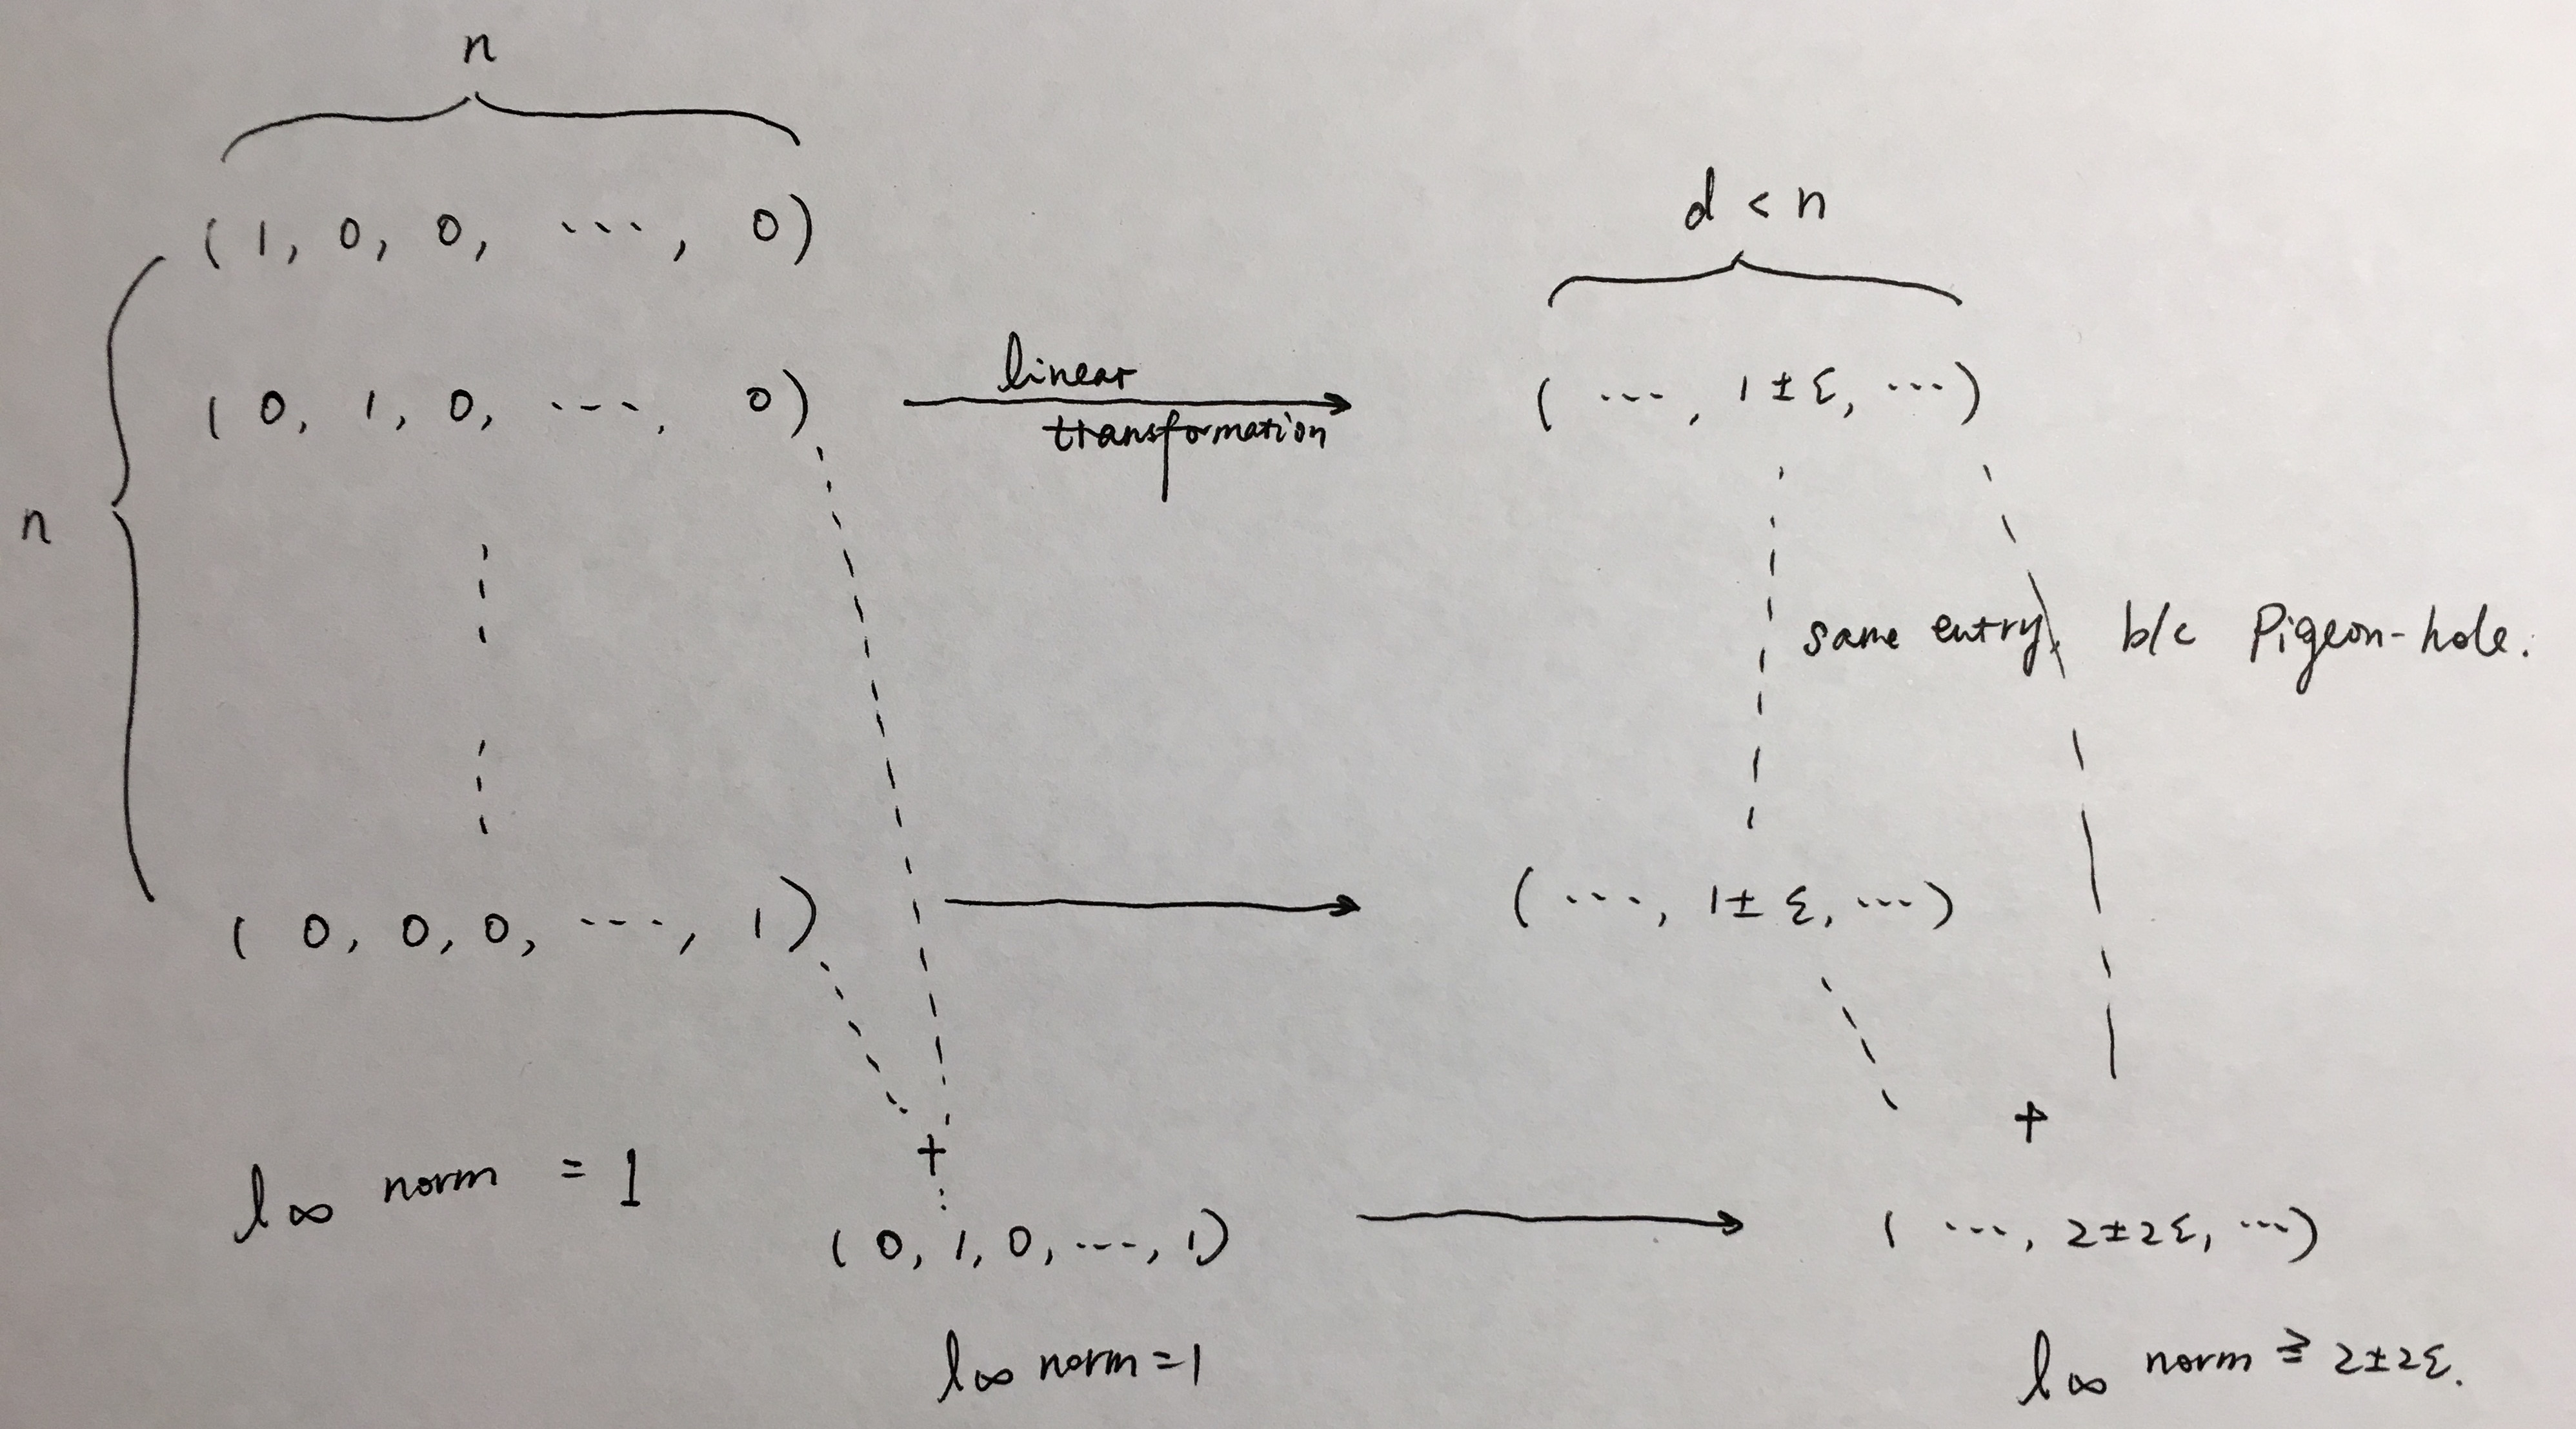
\includegraphics[width=1\textwidth]{6-b.jpg}
	\caption{On the left is $n$ vectors in $\mathbb{R}^n$, with $\ell_\infty$ norm 1, compressed and maps to $n$ vectors in $\mathbb{R}^d$. Solid arrows denote $\ell_\infty$ norm preserving linear transformation. The summation of the two vectors in $\mathbb{R}^n$ that result in entry collision in $\mathbb{R}^d$, show difference in their $\ell_\infty$ norm, thus demonstrated a counter-example.} \label{fig:6-2}
\end{figure}

\paragraph{(c)}
The counter-example of $\ell_1$ norm is constructed using $\ell_\infty$ norm. 
We already showed in (b) that there can't exist $\ell_\infty$ norm preserving linear transformation. Now we construct $\ell_\infty$ from/to $\ell_1$ norm preserving linear transformation. Then we can conclude that $\ell_1$ norm preserving linear transformation can not exist, otherwise we could this 3 linear transformation to compound a $\ell_\infty$ norm preserving linear transformation that we already know does not exist. The illustration is in Figure \ref{fig:6-3}. 

Recall that in (b) we construct a set of 0-1 vectors with $\ell_\infty$ norm 1, and their summations still have $\ell_\infty$ norm 1. We therefore `reverse-engineer' a set of vectors with $\ell_1$ norm 1, also with their summations preserving $\ell_1$ norm 1, in upper left of Figure \ref{fig:6-3}. Notice that to construct a vector satisfying this property, all we need is half 1 and half -1. It can be as many as {$n \choose n/2$} of these vectors. The $\ell_\infty$ from/to $\ell_1$ linear transformation is done by combinatorially $\pm$ all entries in $\mathbb{R}^k$, as sketched using $x, y, z$ in Figure \ref{fig:6-3}. There is indeed an ``exponential blow up'' $2^{k'}$ in this transformation. However, notice that it can be compensated in the sense that this transformation is two-way and the compression step has a ``exponential contraction'' of $O(log\:n)$ (in the lemma). By placing $+$ and $-$ differently in $\mathbb{R}^{n'}$, we can make the max in $\mathbb{R}^n$ spike at different entry through the transformation. Then we can use the argument in (b) again! The Pigeon-Hole principle still applies to $\mathbb{R}^n$. and the notice that summation counter-example we created in (b) still hold (because of $\ell_\infty$ and $\ell_1$ being both 1.). Notice that summation of the half 1 half -1 vector in $\mathbb{R}^{n'}$ still results in\footnote{In a hindsight, this is the key property differs $\ell_1$ norm from $\ell_2$ norm.} $\ell_1$ norm 1. Therefore, if there were existed $\ell_1$ norm preserving linear transformation, there would have existed  $\ell_\infty$ norm preserving linear transformation. Counter-example arises. 
\begin{figure}
	\centering
	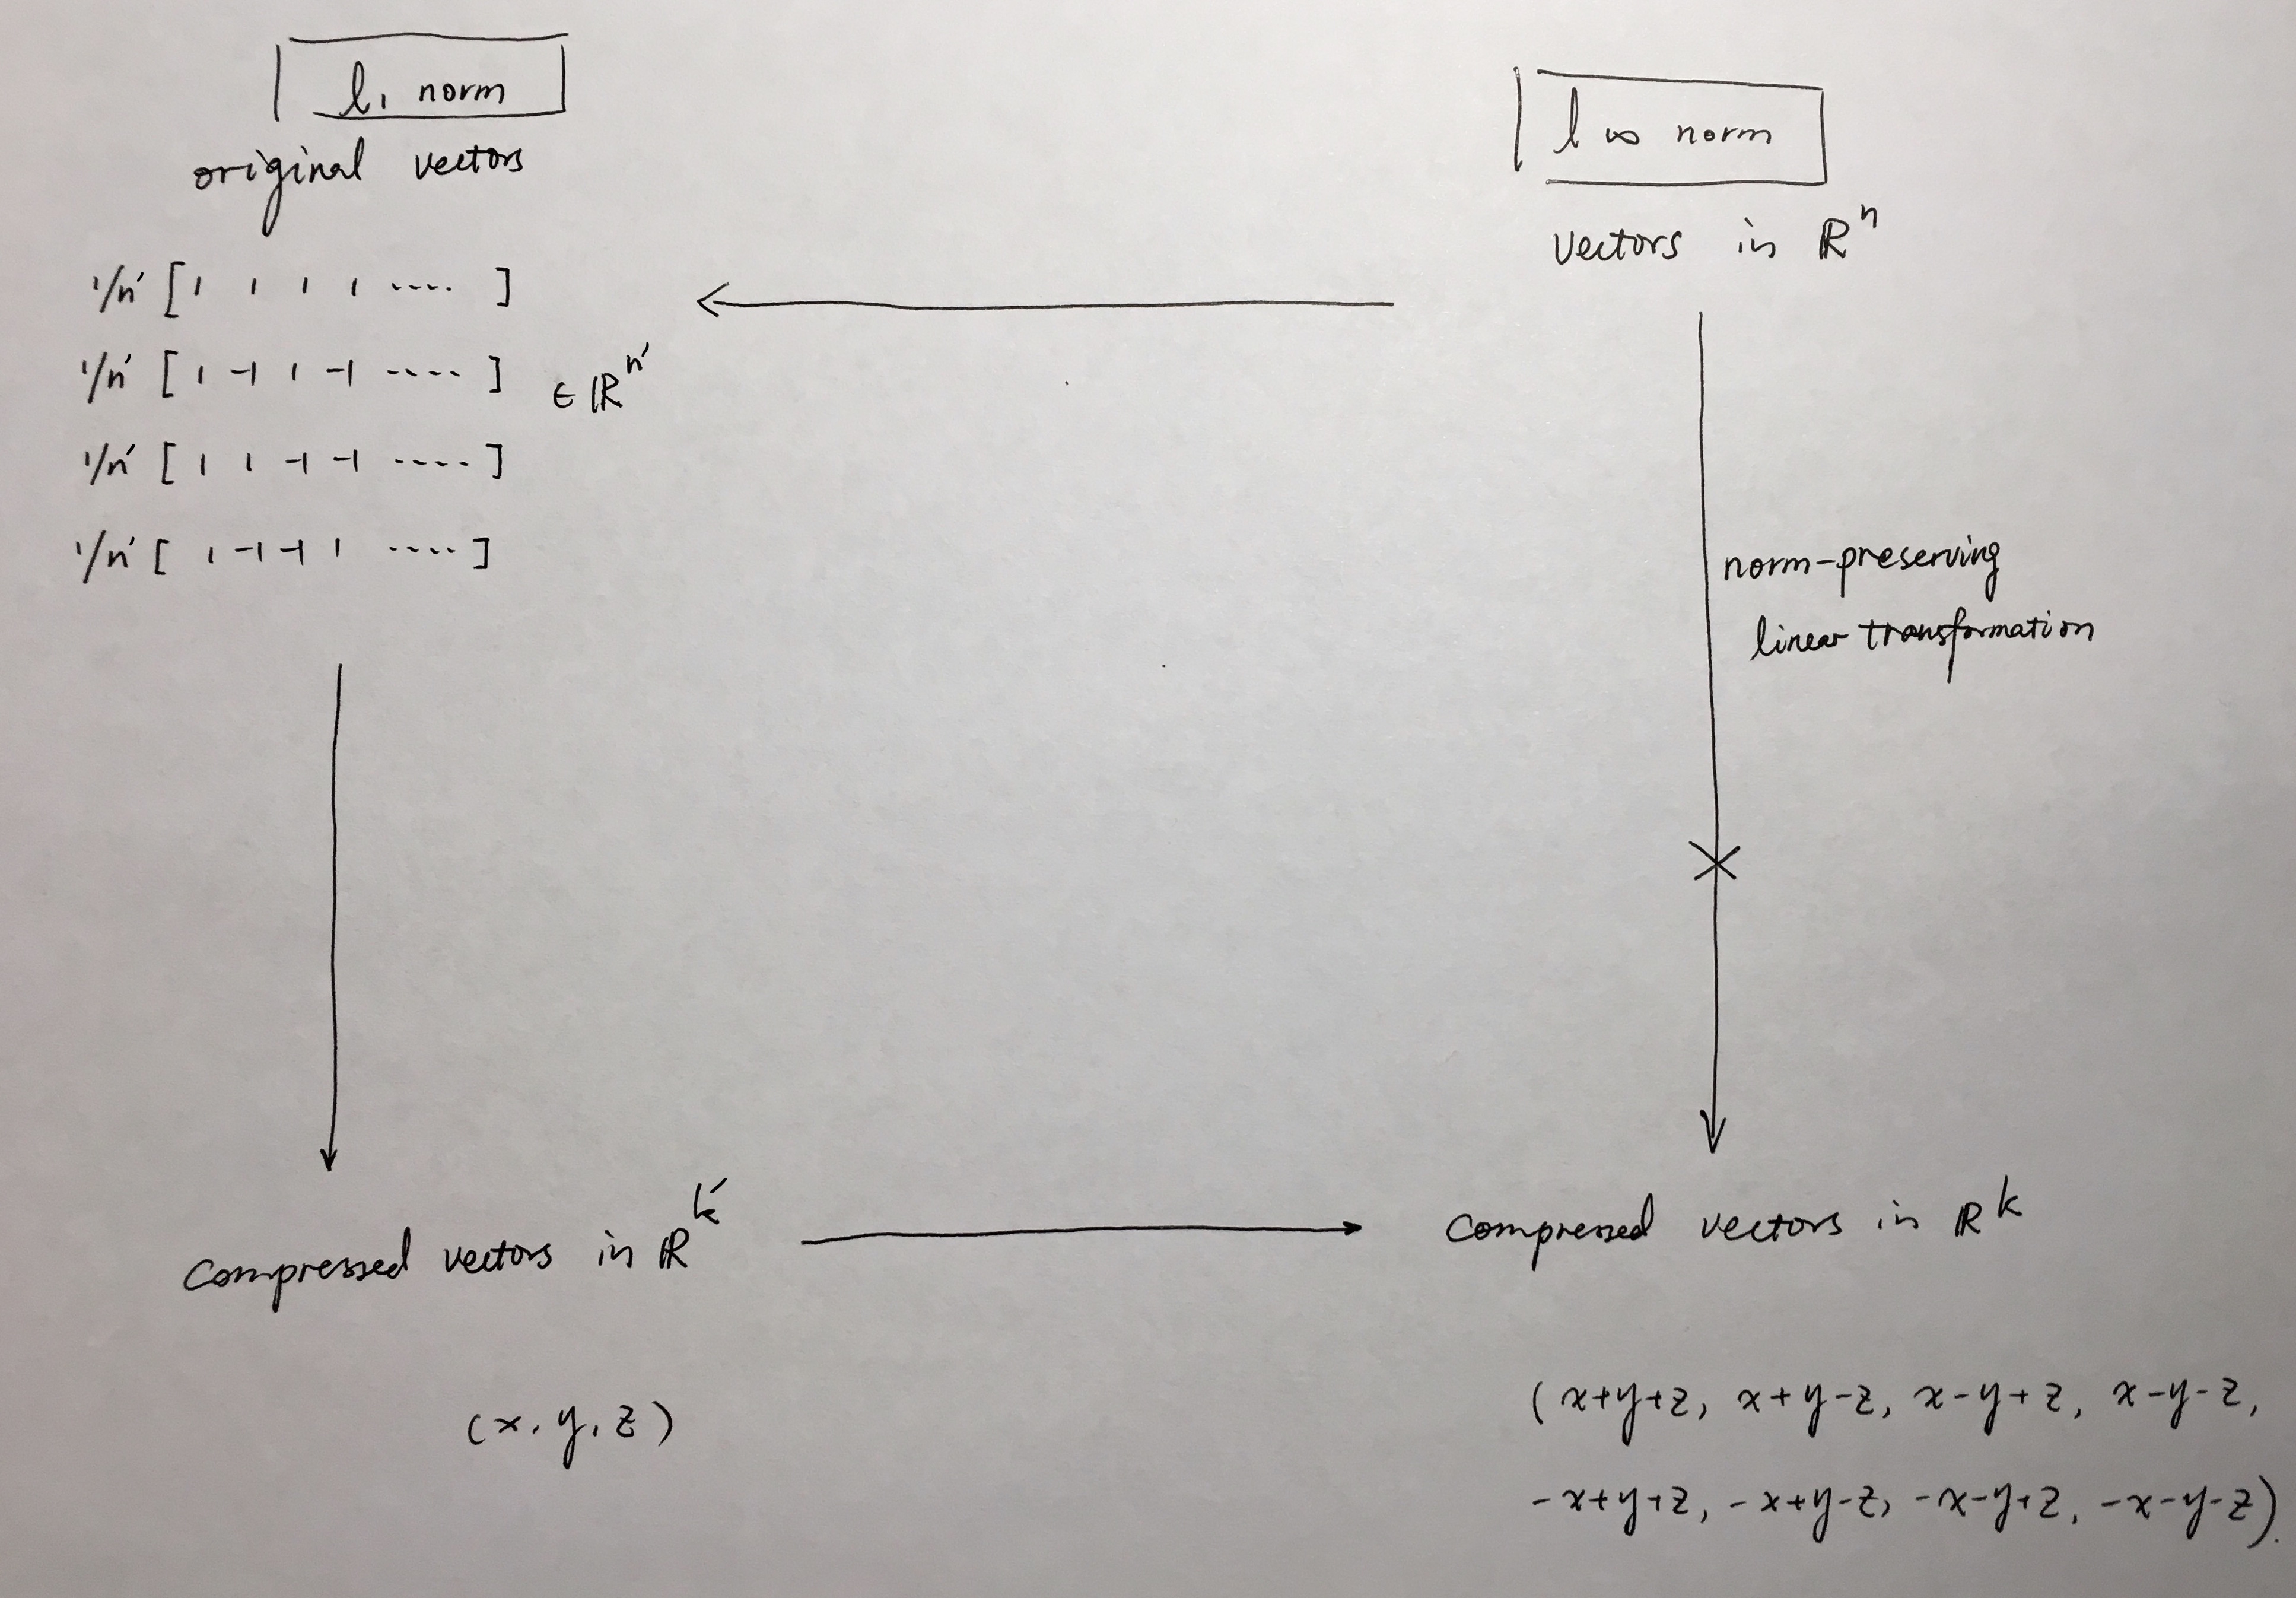
\includegraphics[width=1\textwidth]{6-c.jpg}
	\caption{Transformation graph. Upper right, vectors in $\mathbb{R}^n$ with $\ell_\infty$ equals to 1. Already shown in (b) we know the $\ell_\infty$ norm preserving (down arrow on the right) does not exist in this compression, to lower right, vectors in $\mathbb{R}^k$. The upper and lower two arrows denote the $\ell_\infty$ from/to $\ell_1$ norm preserving transformation over certain vectors. One way of such mapping can be constructed through an example of $x, y, z$. } \label{fig:6-3}
\end{figure}

\end{document}